\chapter{Ergebnisse und Vergleich}
\label{chap:results}

Dieses Kapitel zeigt die Ergebnisse und den Vergleich zwischen den gewöhnlichen state-of-the-art Klassifizierern und den untersuchten RNN-Architekturen. Zunächst wird auf die in den Untersuchungen angewandten Methoden eingegangen, woraufhin die Ergebnisse präsentiert werden.

\section{Angewandte Methoden und Rahmenbedingungen}
\label{section:methods}

Die Experimente verwenden um Vergleichbarkeit sicherzustellen alle denselben in Kapitel 3 beschriebenen ''121 Forearm EMG'' Datensatz. Um eine möglichst hohe Generalisierbarkeit der erzielten Ergebnisse zu erreichen wurden alle Architekturen mittels einer 10-fachen \textit{Cross Validation} evaluiert. Alle Hyperparameter werden aufgrund der rechenintensiven Natur mancher Klassifikatoren manuell optimiert. Die Konfiguration, sowie das Training und die Auswertung der verschiedenen Architekturen geschieht mithilfe der Keras API von Tensorflow und SciKit Learn in der Programmiersprache Python. Das Training erfolgt in der CPU-Version von Tensorflow auf einem Intel 2,3 GHz 8-Kern i9 Prozessor.

Primäte Metriken für den Vergleich der Klassifikatoren sind die Klassifikationsgenauigkeit, sowie die Trainingsdauer. Zunächst werden die gewöhnlichen state-of-the-art Klassifikatoren kNN, SVM, MLP und DT miteinander verglichen und potenzielle Besonderheiten in der Auswertung dieser aufgeführt. Anschließend werden die RNN-Architekturen zunächst miteinander und anschließend mit dem am besten abschneidensten state-of-the-art Klassifikator verglichen, wobei hier ebenfalls auf Besonderheiten in den Ergebnissen und der Auswertung hingewiesen wird.

Im letzten Kapitel erfolgt abschließend ein Fazit der Ergebnisse, sowie ein Ausblick.

\section{Vergleich der gewöhnlichen Klassifikatoren}
\label{sec:other-classifiers-comp}

Beim vergleich der gewöhnlichen Klassifikatoren fällt zunächst auf, dass alle für ihre vergleichsweise simple Architektur bereits gute Ergebnisse erzielen. Im Vergleich zu bisherigen Untersuchungen zu erwarten sind die Ergebnisse der kNN und SVM. kNN sind fürgewöhnlich in Vergleichen die Klassifikatoren mit der geringsten Klassifikationsgenauigkeit \cite{Kaufmann2013}. Trotzdem erreichten kNN in dieser Forschungsarbeit eine ausreichende Genauigkeit in einer vergleichsweise geringen Zeit, was sie zu einem validen Referenzwert macht. SVM erzielten voraussichtlich aufgrund ihrer nativen Minimierung von strukturiertem Risiko und der daraus folgenden geringeren Tendenz zum Overfitting die in Hinblick auf die Klassifikationsgenauigkeit besten Ergebnisse. Gleichzeitig benötigten sie allerdings ebenfalls die zwischen allen state-of-the-art Klassifizierern in dieser Arbeit die mit Abstand längste Trainingsdauer. Die im Rahmen der Arbeit untersuchte MLP Architektur erzielte zwar in einer im Vergleich zu SVM kurzen Zeit vergleichbar präzise Ergebnisse, tat sich allerdings schwer diese selbst mit erhöhter Parameterzahl zu übertreffen. Um die Klassifizierungsgenauigkeit der MLP weiter zu optimieren könnten diesen weitere HL unter sorgsamer Berücksichtigung der Overfitting-Problematik hinzugefügt werden. Eine tiefere Architektur mit zusätzlichen \textit{Dropout}-Schichten zur sicherstellung der Generalisierbarkeit könnte verbesserte Ergebnisse liefern. Ausreißer in diesem Vergleich ist der untersuchte DT. Dieser liefert mit einer Klassifikationsgenauigkeit von 87,13\% eine Präzision nur leicht unter der der SVM in einem Bruchteil der Zeit. Hierzu sei allerdings hinzuzufügen, dass SVM durch weitere Optimierung, wie in vorheriger Forschung bereits zu sehen war \cite{Kaufmann2013} bessere Ergebnisse erreichen und somit die Lücke zwischen DT und SVM vergrößern könnten. 

    \begin{table}[h]
        \centering
        \begin{tabular}{| l | c | c |}
            \hline
            \textbf{Klass.} & \textbf{Acc.} & \textbf{Dur.} \\
            \hline
            kNN & 82,92\% & 02:34 Min.\\ \hline
            SVM & 87,88\% & 07:10 Min.\\ \hline
            MLP & 86,14\% & 03:01 Min.\\ \hline
            DT & 87,13\% & 00:15 Min.\\
            \hline
        \end{tabular}
        \caption{Ergebnisse der Cross Validation aller gewöhnlichen Klassifizierer unterteilt in den verwendeten Klassifizierer (Klass.), die Klassifizierungsgenauigkeit (Acc.) und die Trainingsdauer (Dur.)}
        \label{tab:other-classifiers-comp}
    \end{table}

\section{Vergleich der RNN-Architekturen}
\label{sec:rnn-comp}

Im Fall der untersuchten RNN-Architekturen lassen sich einige Beobachtungen aufstellen. Die prägnanteste Erkenntnis dieses Experiments stellt die Klassifiezierungsleistung der gewöhnlichen RNN auf dem Validierungsdatensatz dar. Trotz weitreichender Optimierung der Hyperparameter und der Verwendung von Techniken wie dem Gradient Clipping erzielten gewöhnliche RNN im Vergleich zu den anderen RNN-Architekturen signifikant schlechtere Ergebnisse. Ihre zuletzt erzielte Klassifikationsgenauigkeit von 82,95\% übertrifft nur marginal die Leistung des kNN Algorithmus auf dem Datensatz. Dieses Ergebnis überrascht vor allem deshalb, weil gewöhnliche RNN in vorigen Untersuchungen auf sEMG Datensätzen bereits gute Ergebnisse erzielten, auch wenn diese im Vergleich zu den LSTM und GRU Architekturen meist dennoch schlechter ausfielen (\cite{simao2019emg}). Da RNN in der Forschung bis jetzt noch nicht mit dem in dieser Arbeit erforschten Datensatz untersucht wurden, könnte eine mögliche Erklärung für dieses Auftreten die länge der Sequenzen sein. Da gewöhnliche RNN häufig unter der Problematik des Vanishing Gradient leiden, die vor allem bei langen Sequenzen zu Fehlklassifikationen führen kann, könnte dieser Schritt die Klassifikationsgenauigkeit stark erhöhen. Der direkteste Indikator für eine vorliegende VG Problematik sind gegen 0 tendierende Gradienten im Netzwerk. Eine VG Problematik könnte anhand des vorliegenden Graphen an der stetigen Abflachung der Klassifikationsgenauigkeit-Kurve erkannt werden, da dies auf geringe Anpassung in den Gewichten der Neuronen und somit auf einen sehr kleinen Gradienten hindeuten könnte. Gleichzeitig lässt sich anhand von Abbildung \ref{rnn-comp} dieser Trend der Abflachung bereits ab der ersten Epoche beobachten. Während die Kurven der LSTM und GRU zunächst konvex verlaufen, ist die Trajektorie der gewöhnlichen RNN konstant konkav. Ein weiteres Indiz für eine VG Problematik lässt sich mit Blick auf die Diskrepanz zwischen der Leistung der gewöhnlichen RNN und den LSTM und GRU Architekturen erkennen. Diese speziell zur Lösung der VG und EG Problematik entwickelten Architekturen liefern nahezu identische Ergebnisse und eine dabei wesentlich höhere Präzision. Da diese Architekturen gewöhnlicherweise keine Schwierigkeiten mit der VG oder EG Problematik haben, könnte dies ebenfalls auf einen VG im Fall der gewöhnlichen RNN deuten. Die direkteste Methode auf eine VG Problematik in den gewöhnlichen RNN zu prüfen wäre das untersuchen der Gradienten während des Trainings des Netzwerks. Tendieren diese gegen 0, liegt VG in der Architektur vor. Allerdings konnte dies aufgrund von technischen Einschränkungen in der verwendeten Tensorflow API im Verlauf dieser Arbeit nicht durchgeführt werden.

Ebenfalls im Vergleich der RNN hervorzuheben ist der Verlauf der LSTM im Verleich zu den GRU. 

\begin{center}
    \begin{tabular}{| l | c | c |}
        \hline
        \textbf{Klass.} & \textbf{Acc.} & \textbf{Dur.} \\
        \hline
        kNN & 82,92\% & 02:34 Min.\\ \hline
        SVM & 87,88\% & 07:10 Min.\\ \hline
        MLP & 86,14\% & 03:01 Min.\\ \hline
        DT & 87,13\% & 00:15 Min.\\
        \hline
    \end{tabular}
\end{center}

\begin{figure}[h]
    \centering
    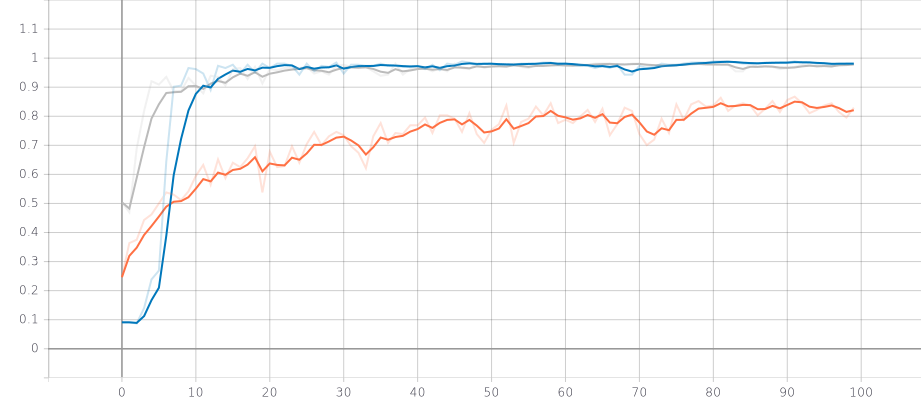
\includegraphics[scale=0.3]{grafiken/rnn-comp.png}
    \caption{Vergleich der Klassifizierungsgenauigkeiten der RNN-Architekturen des gewöhnlichen RNN (Orange), LSTM (Grau) und GRU (Blau)}
    \label{rnn-comp}
\end{figure}